\documentclass[10pt]{article}
\usepackage{amsthm}
\usepackage{amsfonts}
%\usepackage{amsmath}
\usepackage[utf8]{inputenc}
\usepackage{graphicx}
\usepackage{xcolor}
\usepackage[margin=1.0in]{geometry}
\usepackage{fancyvrb}
\usepackage{cprotect}
\usepackage{url}
\usepackage{etoolbox}
\usepackage[hidelinks]{hyperref}
\usepackage[skins,theorems]{tcolorbox}
\usepackage{enumitem}
\usepackage{xcolor}
\usepackage{pifont}
\usepackage{tcolorbox}        % load once, no options
\tcbuselibrary{theorems,skins,breakable} % add features here
%\newcommand*{\vertbar}{\rule[-1ex]{0.5pt}{2.5ex}}
%\newcommand*{\horzbar}{\rule[.5ex]{2.5ex}{0.5pt}}
%\setlist[itemize]{align=parleft,left=1pt..1em}
% \usepackage{tikz}
% \usetikzlibrary{arrows.meta,positioning}
\newcommand{\vertbar}{\,\big|\,}

\usepackage{imakeidx}
\makeindex

\usepackage{listings}
\usepackage{xcolor}

% Define some colors
\definecolor{codegreen}{rgb}{0,0.6,0}
\definecolor{codegray}{rgb}{0.5,0.5,0.5}
\definecolor{codepurple}{rgb}{0.58,0,0.82}
\definecolor{backcolour}{rgb}{0.95,0.95,0.92}

% Define a style
\lstdefinestyle{mystyle}{
    commentstyle=\color{codegreen},
    keywordstyle=\color{blue},
    numberstyle=\tiny\color{codegray},
    stringstyle=\color{codepurple},
    basicstyle=\ttfamily,
    breakatwhitespace=false,
    breaklines=true,
    captionpos=b,
    keepspaces=true,
    numbersep=5pt,
    showspaces=false,
    showstringspaces=false,
    showtabs=false,
    tabsize=4
}

\lstset{style=mystyle}
%\usepackage[T1]{fontenc}
%\usepackage{inconsolata} % optional, nicer monospace font


\usepackage{cmbright}
%\usepackage[OT1]{fontenc}
%\usepackage{helvet}
%\renewcommand{\familydefault}{\sfdefault}

%\usepackage{titlesec}



%\titleformat{\section}
%  {\normalfont\fontsize{14}{17}\sffamily\bfseries}
%  {\thesection}
%  {1em}
%  {}
%
%\titleformat{\subsection}
%  {\normalfont\fontsize{12}{17}\sffamily\slshape}
%  {\thesubsection}
%  {1em}
%  {}



% from https://www.pinterest.co.uk/pin/88664686405122253/
\definecolor{C1}{RGB}{141, 125, 158} %purple
\definecolor{C2}{RGB}{163,156,147} % yellow
\definecolor{C3}{RGB}{99,151,153} % green
\definecolor{C4}{RGB}{195,106,99} % red
\definecolor{C5}{RGB}{124, 132, 128}
\definecolor{C6}{RGB}{67, 69, 75}



\definecolor{Gr}{HTML}{377D71}
\definecolor{Pu}{HTML}{A459D1}
\definecolor{Bl}{HTML}{4D455D}
\definecolor{Te}{HTML}{C1ECE4}
\definecolor{Or}{HTML}{EF6262}
\definecolor{Am}{HTML}{F3AA60}
\definecolor{Co}{HTML}{3C486B}
\definecolor{Wh}{HTML}{FEFBF6}
\definecolor{Ye}{HTML}{FFE196}
\definecolor{Re}{HTML}{E96479}
\definecolor{Pi}{HTML}{FFD0D0}
\definecolor{Rp}{HTML}{FF9EAA}
\definecolor{Wg}{HTML}{EEF3D2}

\newcounter{unit}
\renewcommand{\thesection}{\theunit.\arabic{section}}

\hypersetup{
    colorlinks=false,
    linkcolor=red,
    filecolor=red,      
    urlcolor=red,
    pdftitle={a},
    pdfpagemode=FullScreen,
    }
    
    
 % TCOLORBOX STUFF ----------------------------------------------------------------------------
 

 %  ----------------------------------------------------------------------------
    
%\patchcmd{\section}{\normalfont}{\color{C5}}{}{}
%\patchcmd{\subsection}{\normalfont}{\color{C5}}{}{}


\newcommand{\dfn}[1]{{\underline{#1}}}
\definecolor{sidebarblue}{HTML}{E3F2FD}


\renewcommand{\FancyVerbFormatLine}[1]{\color{gray}{>\,\,#1}}
    
\newtheorem{thm}{Theorem}


\newtheoremstyle{exercise}
{}                % Space above
{}                % Space below
{\color{black}}        % Theorem body font % (default is "\upshape")
{}                % Indent amount
{\bfseries}       % Theorem head font % (default is \mdseries)
{:}               % Punctuation after theorem head % default: no punctuation
{ }               % Space after theorem head
{}                % Theorem head spec
\theoremstyle{exercise}
\newtheorem{exercise}{Exercise}


\newtheoremstyle{example}
  {}                % Space above
  {}                % Space below
  {\color{black}} % Theorem body font (default is "\upshape")
  {}                % Indent amount
  {\bfseries}       % Theorem head font (default is \mdseries)
  {.}               % Punctuation after theorem head (default is no punctuation)
  { }               % Space after theorem head
  {\thmname{#1}\thmnumber{ #2}\thmnote{ \textnormal{(#3)}}}  % Theorem head spec: #1 is name, #2 is number, #3 is note

\theoremstyle{example}
\newtheorem{example}{Example}

% Boxed, breakable 'example' with dashed continuation markers and custom background
	\tcolorboxenvironment{example}{
  enhanced,
  breakable,
  colback=sidebarblue,        % <<< background color
  colframe=black,
  boxrule=1pt,
  arc=5pt,
  left=6pt,right=6pt,top=6pt,bottom=6pt,
  % dashed markers at page breaks
  overlay unbroken={},   % no markers if the box doesn't break
 }

\newtheoremstyle{solution}
{}                % Space above
{}                % Space below
{\color{C5}}        % Theorem body font % (default is "\upshape")
{}                % Indent amount
{\bfseries }       % Theorem head font % (default is \mdseries)
{:}               % Punctuation after theorem head % default: no punctuation
{\newline}               % Space after theorem head
{}                % Theorem head spec
\theoremstyle{solution}
\newtheorem*{solution}{Solution}


\newcommand{\mcS}{\mathcal S}
\newcommand{\mcR}{\mathcal R}
\newcommand{\mcC}{\mathcal C}
\newcommand{\bS}{{\boldsymbol S}}
\newcommand{\bR}{{\boldsymbol R}}
\newcommand{\bC}{{\boldsymbol C}}
\newcommand{\ba}{{\boldsymbol a}}
\newcommand{\bb}{{\boldsymbol b}}
\newcommand{\bs}{{\boldsymbol s}}
\newcommand{\bff}{{\boldsymbol f}}
\newcommand{\br}{{\boldsymbol r}}
\newcommand{\bx}{{\boldsymbol x}}
\newcommand{\bt}{{\boldsymbol t}}
\newcommand{\bv}{{\boldsymbol v}}
\newcommand{\bu}{{\boldsymbol u}}
\newcommand{\bw}{{\boldsymbol w}}
\newcommand{\bc}{{\boldsymbol c}}
\newcommand{\be}{{\boldsymbol e}}
\newcommand{\bq}{{\boldsymbol q}}
\newcommand{\bphi}{{\boldsymbol \phi}}
\newcommand{\brho}{{\boldsymbol \rho}}
\newcommand{\btau}{{\boldsymbol \tau}}
\newcommand{\reals}{\mathbb R}
\newcommand{\ints}{\mathbb N}
\newcommand{\E}{\mathbb E}
\newcommand{\Prob}{\mathbb P}


\newcommand{\sectionrefs}[1]{\par\smallskip\noindent\textbf{References:} #1\par\smallskip}


%%%%%%%%%%%%%%%
% adding space between items
%\usepackage{enumitem}
%\setlist{topsep=1.5em, itemsep=1.1em}




%--------------------------------------------------------------------------------------------------------------------------------
\setcounter{unit}{3}
\setcounter{section}{0}

\begin{document}

\title{Unit 3: Statistical inference and single-predictor linear regression models}
\author{Ethan Levien}
\maketitle
\tableofcontents



\newif\ifhideproofs
%\hideproofstrue %uncomment to hide proofs

\ifhideproofs
\usepackage{environ}
\NewEnviron{hide}{}
\let\proof\hide
\let\endproof\endhide
\fi






\section{Introduction}


Now we are almost ready to begin working with regression models, but we first discuss some concepts from statistical inference. These include the idea of a sample distribution (already alluded to in our discussion of the central limit theorem), bias, consistency and confidence intervals. Then we work define lienar regression models, which have also already appeared in different forms.    The basic idea is that we have some predictors $X_1,X_2,\dots,X_k$ and conditional on these variables, the distribution of another variable -- the response variable $Y$ -- is Normal. Moreover, it's mean is a linear function of these variables. These two assumptions allow us to obtain relatively simple formula (at least for a computer) for the coefficients of the $X_i$ in the linear formula. We will start, in this section, with a single-predictor learn how to access a linear regression model in this context. In particular, we will learn about correlation coefficients, $R^2$ and $p$-values, standard errors, confidence intervals. You will need to understand what all these quantities tell us and how they are related. 





\section{Estimators}
We have danced around the concept of statistical inference and parameter estimation for a bit and we saw an example of an estimator: $\hat{q} = \overline{Y}$ is an estimator of the parameter $q$ for a Bernoulli distribution.  We also talked a lot about going between the world of data (e.g. sample means, histogram) and math (e.g. expectation, density) with sample averages. W
{\bf Statistical inference is the process of estimating the parameters (e.g. $\mu$ and $\sigma$) based on samples of $Y$ AND expressing our uncertainty in these estimates.} The expressing the uncertainty part is what we have not yet discussed formally. 


In general, an \dfn{estimator} $\hat{\theta}$  of a parameter $\theta$ is just something we compute from the data which is meant to approximate $\hat{\theta}$. This could in principle be any quantity we can compute from the data (like the maximum value), but it will almost always be represented as a sample average in some way. We will see examples of this soon. 

The point that should be emphasized is that the estimator is a function of the data. That is, {\bf $\hat{\theta}$ depends on the specific data we collect} or simulation we run. It is meant to approximation a parameter which does not depend on the data and is (in classical statistics) a fixed number. For example,  in the instance of a YES/NO survey or election with two candidates, the ``true'' quantity we are interested in measuring is the fraction of people answering YES to some question. Our estimate, $\hat{q}$, is a variable which depends on the specific subset of the population we sample and it will change if we look at a different subset. 



\subsection{Sample distribution and standard errors}
 We call the distribution of $\hat{\theta}$ over many replications of our data the \dfn{sample distribution}. I will use \dfn{replicate} to mean different realizations of our data (as opposed to the different samples within the data). The distinction is shown in Figure \ref{fig:reps_samp} (left panel). The terminology gets a bit confusing: The sample distribution is the distribution of $\hat{\theta}$ over many replicates, but each replicate involves many samples. 

\begin{figure}[h]
\centering
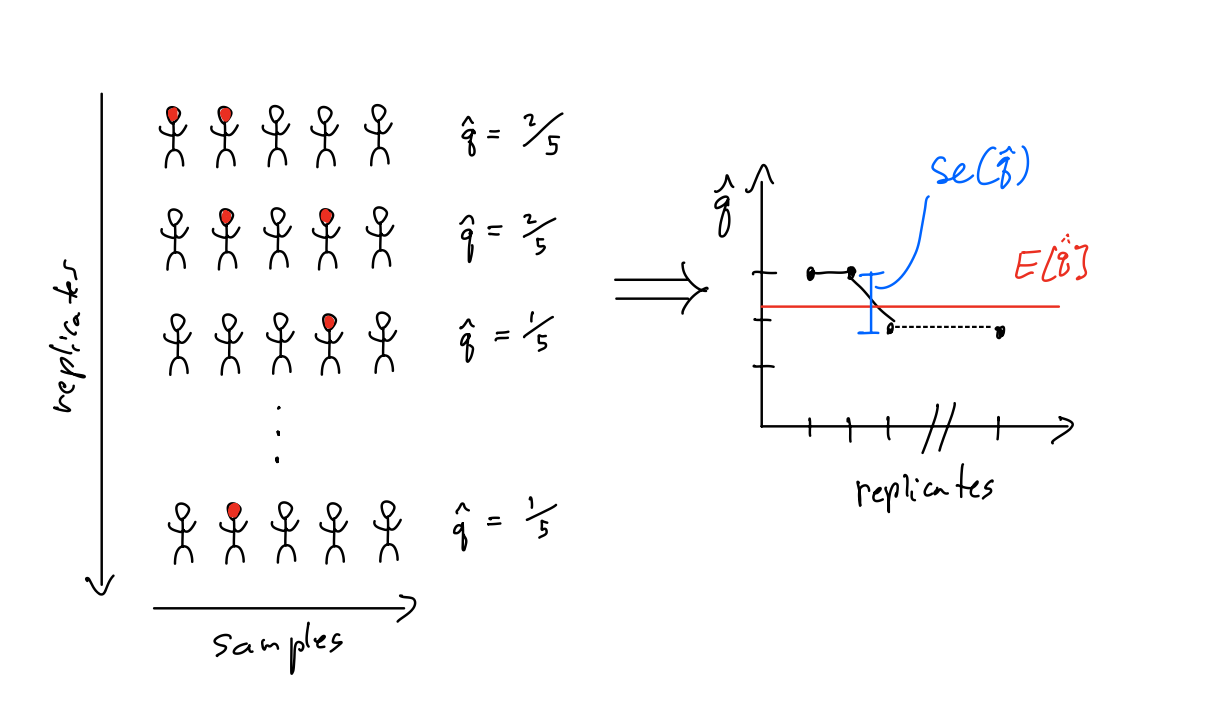
\includegraphics[width=0.8\textwidth]{./../figures/replicates}
\caption{Replicates and samples }\label{fig:rep_samp}
\end{figure}


\begin{example}[sample distribution of normal mean]
Suppose 
\begin{equation*}
Y \sim {\rm Normal}(\mu,\sigma)
\end{equation*}


\noindent
\underline{Question:} What is the sample distribution of $\hat{\mu}$ (our estimate of $\mu$)?\\

\noindent
\underline{Solution:}
\begin{equation*}
\hat{\mu} = \bar{Y} = \frac{1}{N}\sum_{i=1}^NY_i
\end{equation*}
The CLT tell us (informally speaking) that 
\begin{equation*}
\sum_{i=1}^NY_i \sim {\rm Normal}\left(\mu n,n\sigma^2 \right)
\end{equation*}
where by $\sim$ we really mean ``approximately distributed as''. Dividing by $N$, 
\begin{equation*}
\hat{\mu} \sim {\rm Normal}\left(\mu ,\frac{\sigma^2}{N} \right)
\end{equation*}
This assumes $\sigma$ is known.

\end{example} 

 A natural way to quantify the uncertainty in our estimate is the standard deviation of the $\hat{\mu}$ under the sample distribution.  We call the resulting quantity the \dfn {standard error}, which is our \dfn{estimate} of the standard deviation of the sample distribution.  For the Normal model, if we are estimating the mean and happen to know $\sigma$, then 
\begin{equation}\label{eq:se1}
{\rm se}(\hat{\mu}) =  \frac{\sigma}{\sqrt{N}}. 
\end{equation}
This tells us how much our estimate will vary between different experiments (or surveys/simulations). 
Importantly, the standard error depends on $\sigma$ which we may not know!!! Thus, it is common to estimate the standard error using an estimate of $\sigma$, $\hat{\sigma}$, leading to an estimator of the standard deviation:
\begin{equation}\label{eq:se2}
{\rm se}(\hat{\mu}) =  \frac{\hat{\sigma}}{\sqrt{N}}. 
\end{equation}
It should be clear from the context which one we are talking about: If we are working with data and we don't know what $\sigma$ is, when we say standard error we mean Equation \ref{eq:se2}. If we are working with a particular model where we have specified the parameters, we mean Equation \ref{eq:se1}. 







\subsection{Bias and consistency}

 There must be some properties we would like the estimator to have. At a minimum, it should be in some way informed by the data, in the sense that having more data should bring our estimate closer to the actual value of the parameter. More precisely, the more data we have (e.g. the larger $N$) the closer we expect $\hat{\theta}$ to be to the true value $\theta$. Of course, we must define what we mean by "closer" when we are talking about random things. 
For our purposes we will say $\hat{\theta}$ is \dfn{consistent} if 
\begin{equation*}
E[\hat{\theta}] \to \theta\,\,\text{ and } {\rm se}(\hat{\theta})  \to 0 \,\,\,\text{ as }\,\, N\to \infty. 
\end{equation*}
This is saying that as we obtain more and more samples, the sample distribution because more concentrated around $\theta$. 


To see that consistency is not the only property we look for in an estimator, notice that since $\hat{\mu}_1 = \hat{\mu} + 1/N$ is also consistent, yet clearly seems inferior to $\hat{\mu}$. To this end, we say that an estimator $\hat{\theta}$ is \dfn{unbiased} for some $N$ (not just very large $N$), the average over the sample distribution is equal to the actual value under the model distribution; that is, 
\begin{equation*}
E[\hat{\theta}] = \theta. 
\end{equation*} 

\begin{example}[Bias and consistency]
For a normal random variable, define the following estimators of the mean:
\begin{align*}
%\hat{\mu}_1 &= \frac{1}{N}\sum_{i=1}^NY_i + \frac{1}{N}\\
\hat{\mu}_2 &= \frac{Y_1 + Y_2}{2}
\end{align*}

\noindent
\underline{Question:}  Is $\hat{\mu}_2$ biased and consistent? what is the sample distribution?\\


\noindent
\underline{Solution:}
%Note that  $\hat{\mu}_1 = \hat{\mu} + 1/N$ so it has the sample distribution  
%\begin{equation*}
%\hat{\mu}_1 \sim {\rm Normal}(\mu+1/N,\sigma/\sqrt{N})
%\end{equation*}
%while 
Note that $\hat{\mu}_2$ has the sample distribution 
\begin{equation*}
\hat{\mu}_2  \sim {\rm Normal}(\mu,\sigma/\sqrt{2})
\end{equation*}
\end{example}


\begin{example}[Normal standard deviation]
Let now consider estimating the standard deviation of a Normal random variable
\begin{equation*}
Y \sim {\rm Normal}(\mu,\sigma^2)
\end{equation*}
Given samples $Y_1,Y_2,\dots,Y_n$, it seems the natural way to estimate $\sigma^2$ is using
\begin{equation*}
{\rm var}(Y) = E[(Y-E[Y])^2] \approx \frac{1}{n}\sum_{i=1}^n(Y_i-\overline{Y})^2
\end{equation*}
we will call this estimator $\hat{\sigma}_0^2$. It turns out $\hat{\sigma}_0^2$ is biased and in-fact 
\begin{equation*}
\hat{\sigma}^2 = \frac{1}{n-1}\sum_{i=1}^n(Y_i-\overline{Y})^2 = \frac{n}{n-1}\hat{\sigma}_0^2
\end{equation*}
is unbiased. The correction by a factor $n/(n-1)$ is called Bessel correction. \\

\noindent
\underline{Question:} Demonstrate with simulated data that $\hat{\sigma}_0^2$ is biased and $\hat{\sigma}^2$ is not. 


\end{example}






\subsection{Confidence intervals}


The idea of the \dfn{confidence interval} is, roughly speaking, to describe the range of values where we think the actual value of $\theta$ might reasonable be given some estimate $\hat{\theta}$ and its sample distribution. We will mostly work with the $95\%$ \dfn{ confidence interval}, or $95\%$-CI, which is given by 
\begin{equation}\label{eq:95CI}
[\hat{\theta} - 1.96{\rm se}(\hat{\theta}), \hat{\theta} + 1.96{\rm se}(\hat{\theta})]
\end{equation}
The factors $1.96$ in front of the standard errors ensure that $95\%$ of samples from the sample distribution will fall in this range, 



Note that these samples from the sample distribution do not have the same distribution as $\hat{\theta}$ over replicates of our data. Said another way, if we draw many samples from our estimate of the sample distribution, their distribution will not be the same as the distribution of $\hat{\theta}$ we would obtain if we ran an experiment many times and estimated $\hat{\theta}$ each time. The correct interpretation of the $95\%$-CI is as follows: {\bf If we generate many replicates of the data then $\theta$ (the true value) will fall in the CI, for $95\%$ of them.} 

Technically speaking, is is NOT the case that there is a $95\%$ chance the true value of $\theta$ is in the $95\%$-CI. 
To understand why, note that the parameter has a $95\%$ chance to be in the interval 
\begin{equation}\label{eq:95CIB}
[\theta - 1.96{\rm std}(\theta),\theta + 1.96{\rm std}(\theta)]
\end{equation}
but this is difference from Equation \ref{eq:95CI}, since we have replaced $\hat{\theta}$ with $\theta$. The distinction, which is shown in Figure \ref{fig:CI}, is important; however, you don't need to get bogged down by the subtle differences in interpretation. For practical purposes, you can pretty much thing of the $95\%$-CI as the region where the parameter value is likely to be. We provide alternatives ways to think about these intervals when we discuss Bayesian vs. classical statistics. 


\begin{figure}[h]
\centering
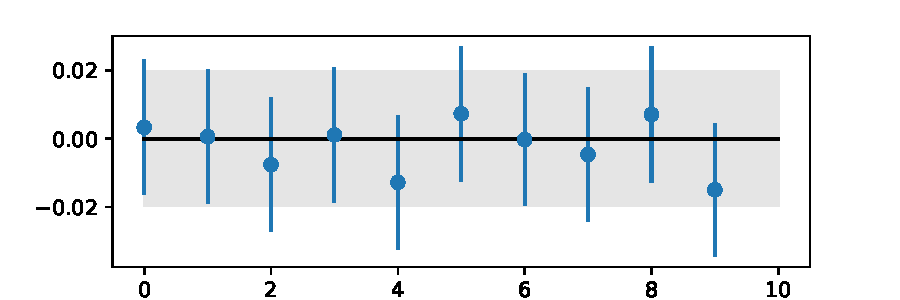
\includegraphics[width=0.8\textwidth]{./../figures/notes3CI}
\caption{An illustration of the distinction between Equation \ref{eq:95CIB} (gray shaded region) and Equation \ref{eq:95CI}.   }\label{fig:CI}
\end{figure}

\begin{example}[Estimating CI]
% NEED BETTER MOTIVATION
Imagine we are designing an experiment. Our model is a Normal distribution and from previous experience, we have a ballpark estimate of the standard deviation, which is $\sigma \approx 0.1$.  \\



\noindent
\underline{Question:} Roughly, how many samples do we need to collect to have a $95\%$ chance our estimate is within $0.1$ of the actual value of the variable?\\



\noindent
\underline{Solution:} The standard deviation of an estimate based on $n$ samples will have a confidence interval of 
\begin{equation*}
[\hat{\mu}-0.196/\sqrt{n},\hat{\mu} +  0.196/\sqrt{n}]
\end{equation*}
The width of this interval is $2 \times 0.196/\sqrt{n}$. This interval will intersect the true value in $95\%$ of replicates, so we would like it to have a width $<0.2$. It follows that we need 
\begin{equation*}
1.96^2 = 3.8 < n 
\end{equation*}
We can test this by running many replicates for each $n$, as done in the class notebook. 
% Make a plot of the sample fraction of samples with $0.1$ of the actual mean as a function of the number of samples to confirm the result of part (a)
\end{example}




%\begin{exercise}
% \href{https://colab.research.google.com/drive/1QarJhwPmSqCTQ-HwU_lXCUX6uvdhLdrM#scrollTo=US27cD1JgXn_&line=3&uniqifier=1}{Understanding bias}
%\end{exercise} 



%------------------------------------------------------------------------------------------------------------------------------------------------------
\subsection{Bias-variance tradeoff}

We introduce the \dfn{mean-squared error} of an estimator $\hat{\theta}$ of some quantity $\theta$. $\theta$ could be a parameter, or it could be a value of a function, such as $f(x)$, that we would like to predict. 
\begin{equation}\label{eq:mse}
{\rm MSE}_{\hat{\theta}}= E\left[(\hat{\theta}- \theta)^2\right]
\end{equation}
 For now, let's just think of $\hat{\theta}$ as any estimator. 
The following theorem is the key result which will allow us to understand the U-shaped curve. 
\begin{thm}[Bias variance decomposition]
\begin{equation}\label{eq:biasvar}
{\rm MSE}_{\hat{\theta}} = {\rm var}(\hat{\theta}) + E\left[\hat{\theta}-\theta\right]^2
\end{equation}
\end{thm}
\begin{proof}
Using the definition of variance 
\begin{equation*}
{\rm var}\left(\hat{\theta}-\theta\right) = E\left[(\hat{\theta}-\theta)^2\right] - E\left[\hat{\theta}-\theta\right]^2. 
\end{equation*}
Since $\theta$ is a constant, ${\rm var}\left(\hat{\theta}-\theta\right)= {\rm var}\left(\hat{\theta}\right)$, so 
rearranging terms yields the result. 
\end{proof}


%------------------------------------------------------------------------------------------------------------------------------------------------------
\subsection{Maximum Likelihood (optional)}

Sometimes it is quite clear what the estimator for a parameter should be. This is the case for $q$ in the Bernoulli distribution. However, we will find this is not always the case, so it is useful to have a {\bf more systematic way of finding estimators.} 
Recall that the probability distribution for the binomial distribution is 
\begin{equation}\label{eq:binomial-pdf}
p(Y) = {n \choose Y}q^Y(1-q)^{n-Y}
\end{equation}
In statistics, we sometimes call this the \dfn{likelihood} and denoted $P(Y) = L(Y|q)$. The notation here is suggesting that we think of $P$ as a distribution which is conditioned on a particular value of the parameter.  More generally, the likelihood is defined as the probability we say a data set given the parameters. This notation and terminology foreshadows Bayesian thinking, wherein one thinks of the parameter as random variables themselves -- more on this later. 
For now, notice that Equation \eqref{eq:binomial-pdf} tells us how likely it is to observe $k$ YES among $n$ people surveyed. Then, it seems reasonable that this number should not be very small, since that would mean our survey results are an anomaly. More generally, the larger $L(Y|q)$ is the more likelihood our results are. This suggests one a way to estimate determine $q$: We can take as our estimate $\hat{q}$ the value which makes $L(Y|q)$ largest. In other words, we are finding the value of $q$ which makes the data the most likely, and we will call this the \dfn {maximum likelihood estimate}.
You can do this using calculus (if you know how, I suggest you give it a try) to determine that the value of $q$ which makes \eqref{eq:binomial-pdf} largest is \begin{equation*}
\hat{q}_{\rm MLE} = \frac{Y}{n}
\end{equation*}
For a Normal distribution with mean and variance $\mu$ and $\sigma$, the MLE estimators are the usual sample mean and standard deviation which we have already been exposed to. 

\section{Single-predictor linear regression model}
Regression models model input-output relationships. The input is the \dfn{predictor} ($X$) and the output is the \dfn{response} variable ($Y$). For a  \dfn{linear regression model}, 
\begin{align*}
Y = \beta_0 + \beta_1 X_1 + \epsilon,\quad \epsilon \sim {\rm Normal}(0,\sigma_{\xi}^2).
\end{align*}
Written another way
\begin{equation}
Y|X \sim {\rm Normal}(\beta_0 + \beta_1 X,\sigma^2). 
\end{equation}
It should be noted that in regression modeling the distribution of the predictor is often not specified. However, we should always think about what this is, because it plays an important role in the inference process as I will discuss below. For this reason, I often think of a linear regression model as a model of both variables:
\begin{align}
\begin{split}\label{eq:linreg}
X &\sim \text{some distribution with mean $\mu_x$ and variance $\sigma_x^2$}\\
Y|X &\sim {\rm Normal}(\beta_1X + \beta_0,\sigma^2). 
\end{split}
\end{align}
In the examples below we look at Bernoulli and Normal predictors. 
 

 \begin{example}[Linear regression with a binary predictor: the difference of means]\label{ex:zerothreg}
 Let
\begin{align*}
X &\sim {\rm Bernoulli}(q)\\
Y|X &\sim {\rm Normal}(\beta_1X + \beta_0,\sigma^2)
\end{align*} \noindent
\underline{Question:} What is the marginal mean of $Y$? What is an estimator of $\beta_1$? (not using covariance as below)  Is it biased? \\


 \noindent
\underline{Solution:} 


 \end{example}

 
 \begin{example}[Linear regression model with Normal predictor]\label{ex:firstreg}
Let
\begin{align*}
X &\sim {\rm Normal}(\mu_x,\sigma_x^2)\\
Y|X &\sim {\rm Normal}(\beta_1X + \beta_0,\sigma^2)
\end{align*}

 \noindent
\underline{Question:} What is the marginal distribution of $Y$? What is $E[XY]$? How does this compare to $E[X]E[Y]$?\\


 \noindent
\underline{Solution:} We know that 
\begin{equation*}
Y|X =\beta_1X+\beta_0 + Z,\quad Z \sim {\rm Normal}(0,\sigma^2)
\end{equation*}
Thus, the marginal distribution of $Y$ is the sum of two Normal random variables with mean and variance $(\beta_1\mu_x+\beta_0,a\sigma_x^2)$ and $(0,\sigma^2)$ respectively. 
By Theorem \ref{thm:addingnormal}, 
\begin{equation*}
Y  \sim {\rm Normal}(\beta_1\mu_x+\beta_0,\beta_1^2\sigma_x^2 + \sigma^2)
\end{equation*}

To compute $E[XY]$, we note that 
\begin{equation*}
E[XY|X=x]=  E[xY|X=x]= xE[Y|X=x]
\end{equation*}
therefore
\begin{equation*}
E[XY] = E[XE[Y|X]] = E[X(\beta_1X+\beta_0)] = \beta_1E[X^2]+\beta_0E[X]
\end{equation*}
Using 
\begin{equation*}
E[X^2] = {\rm var}(X) + E[X]^2 = \sigma_x^2 + \mu_x^2
\end{equation*}
Therefore 
\begin{equation*}
E[XY] =  \beta_1\sigma_x^2 + \beta_1\mu_x^2 + \beta_0\mu_x
\end{equation*}
On the other hand, 
\begin{equation*}
E[X]E[Y] = \mu_x(\beta_1\mu_x+\beta_0) = \beta_1 \mu_x^2 +\beta_0 \mu_x
\end{equation*}
The difference between the two is the additional term $\beta_1\sigma_x^2$, which we picked up from the variance of $x$.  


\end{example}


\subsection{Covariance} 
 The example above motivates the definition of \dfn{covariance}
\begin{equation}
{\rm cov}(X,Y) = E[XY]-E[X]E[Y]
\end{equation}
Note that another way to write this is 
\begin{equation*}
 E[(Y-E[Y])(X-E[X)] = E[XY] - 2E[X]E[Y]+E[X]E[Y] = {\rm cov}(X,Y)
\end{equation*}
so if we replaced $X$ with $Y$, this becomes the variance. 
 
 
The relationships above can easily be generalized. 
Recall that we can write $E[X^2]$ as
\begin{equation*}
E[X^2] ={\rm var}(X) + E[X]^2 =  \sigma_x^2 + \mu_x^2. 
\end{equation*}
Now for any linear regression model
\begin{align*}
E[XY] &= E[XE[Y|X]] = E[X(\beta_1 X+\beta_0)] = \beta_1E[X^2] + \beta_0 E[X] \\
&= \beta_1\sigma_x^2 +\beta_1 \mu_x^2 +\beta_0 \mu_x\\
E[Y] &= \beta_1\mu_x +\beta_0
\end{align*}
so 
\begin{align*}
{\rm cov}(X,Y) &= \beta_1\sigma_x^2
\end{align*}
regardless of the distribution of $X$ (assuming $\sigma_x^2 <\infty$). The intuition for this formula is given in figure \ref{fig:cov_effect}.


\begin{figure}[h]
\centering
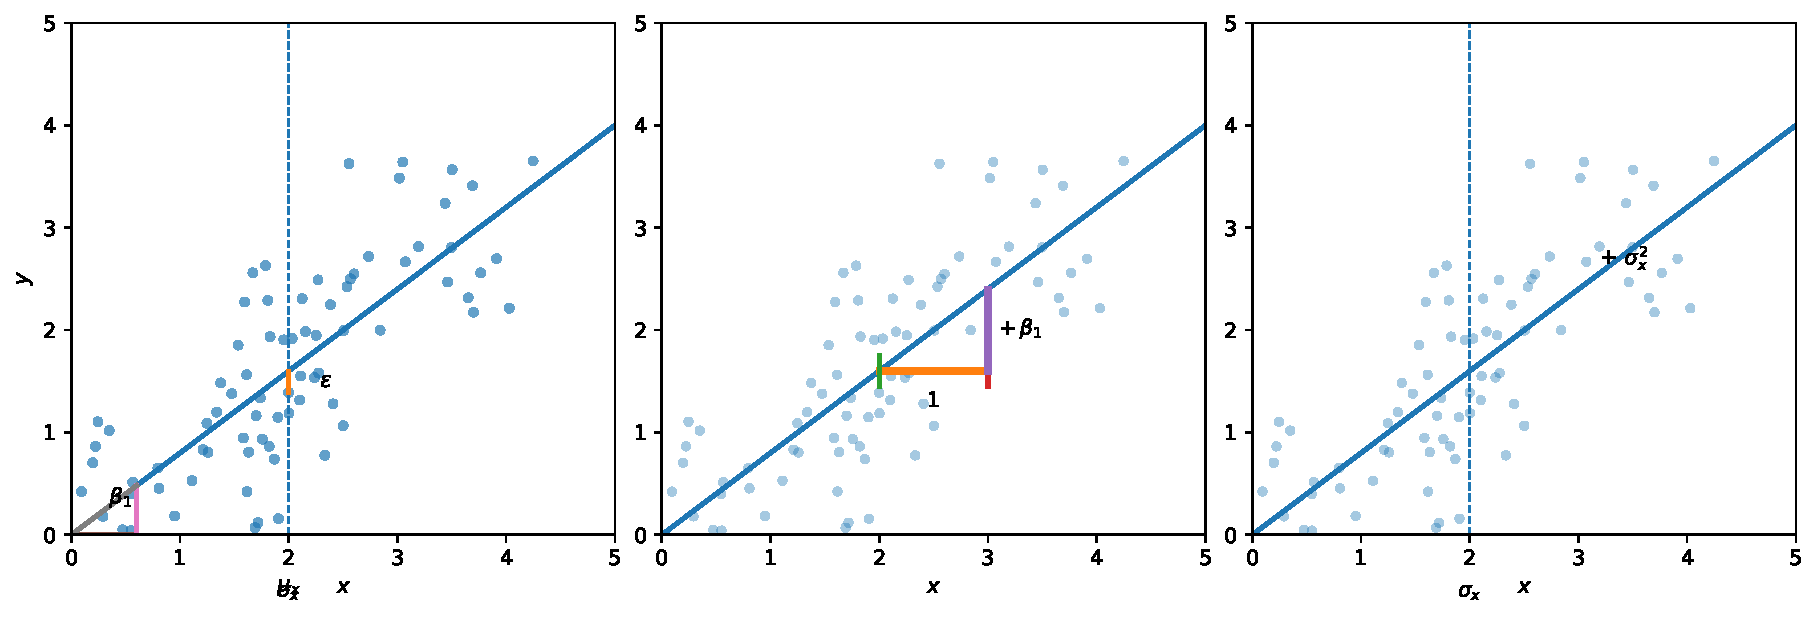
\includegraphics[width=0.8\textwidth]{./../figures/cov_effect}
\caption{}\label{fig:cov_effect}
\end{figure}


A crucial observation is that the covariance allows us to relate the parameter $\beta_1$ (the slope) in the model above to averages over $X$ and $Y$. In other words, it provides us with a means to estimate the slope from samples $(x_1,y_2),\dots,(x_n,y_n)$. 
\begin{align*}
 \beta_1 &\approx  \frac{\sum_{i=1}^n\left(x_i - \bar{X}\right)\left(y_i-\bar{Y}\right)}{\sum_{i=1}^n\left(x_i - \bar{X}\right)^2}
\end{align*}
The is what the function 
\begin{Verbatim}
np.cov(x,y)[0,1]
\end{Verbatim}
computes in Python. 
The reason for the $[0,1]$ is that the covariance function in numpy actually computes a 2D array (a Matrix), where the off diagonal entries are the covariance. The diagonal entries are the variances. 

We can also estimate $\beta_0$. Using $E[Y] = \beta_1 \mu_x + \beta_0$ we have
\begin{equation*}
\beta_0 =  E[Y]  - \beta_1 \mu_x \approx \hat{\beta}_0 =  \overline{Y} - \left(\frac{\sum_{i=1}^n\left(x_i - \bar{X}\right)\left(y_i-\bar{Y}\right)}{\sum_{i=1}^n\left(x_i - \bar{X}\right)^2}\right)\overline{X}
\end{equation*}



\subsection{Least square interpretation}
 Suppose we plot $X$  and $Y$ points in a place. Regardless of where these $X$ and $Y$ points come from (Normal model or not), we can compute $\hat{\beta}_1$ and $\hat{\beta}_0$. 
These estimators are known as \dfn{least squares} estimators (note that we haven't formally defined what an estimator is) because  it happens that these values minimize the sum of the squared difference between our data points and the line $\hat{a}x + \hat{b}$. That is, they are the values that make the \dfn{residual sum of squares}(RSS) smallest
\begin{equation*}
RSS = \sum_{i=1}^n r_i^2,\quad r_i  = Y_i - (\hat{\beta}_1X_i + \hat{\beta}_0)
\end{equation*}
smallest. The R

%\begin{tikzpicture}[>=Stealth, line cap=round, line join=round, scale=1.1]
%
%% Parameters for the regression line: y = m x + b
%\def\m{0.7}
%\def\b{0.5}
%
%% Axes
%\draw[->] (0,0) -- (5.4,0) node[below] {$X$};
%\draw[->] (0,0) -- (0,3.9) node[left] {$Y$};
%
%% Regression line
%\draw[very thick, red] (0,\b) -- (5,\m*5+\b);
%
%% Data points: (xi, yi). Adjust as desired.
%%             i   x     y
%\foreach \i/\x/\y in {
%  1/0.7/0.35,
%  2/1.5/0.95,
%  3/2.3/1.05,
%  4/3.2/1.55,
%  5/4.1/1.85
%}{
%  % Predicted value on the line at x: yhat = m*x + b
%  \pgfmathsetmacro{\yhat}{\m*\x+\b}
%  % Residual segment (vertical): from (x, y) to (x, yhat)
%  \draw[red, line width=1pt] (\x,\y) -- (\x,\yhat);
%  % Residual label r_i near the middle of the segment
%  \pgfmathsetmacro{\ymid}{(\y+\yhat)/2}
%  \draw[red] (\x+0.08,\ymid) node {$r_{\i}$};
%
%  % Data point
%  \fill (\x,\y) circle (1.5pt);
%  % Label y_i next to the point
%  \node[anchor=east] at (\x-0.08,\y) {$y_{\i}$};
%  % Optional: label \hat y_i near the line (comment out if not wanted)
%  % \node[red, anchor=south] at (\x,\yhat) {$\hat y_{\i}$};
%}
%
%% Annotation: minimize sum of squared residuals
%\node[red] at (2.6,0.9) {$\displaystyle \min_{a,b}\ \sum_{i} r_i^{\,2}$};
%
%\end{tikzpicture}
\begin{figure}[h]
\centering
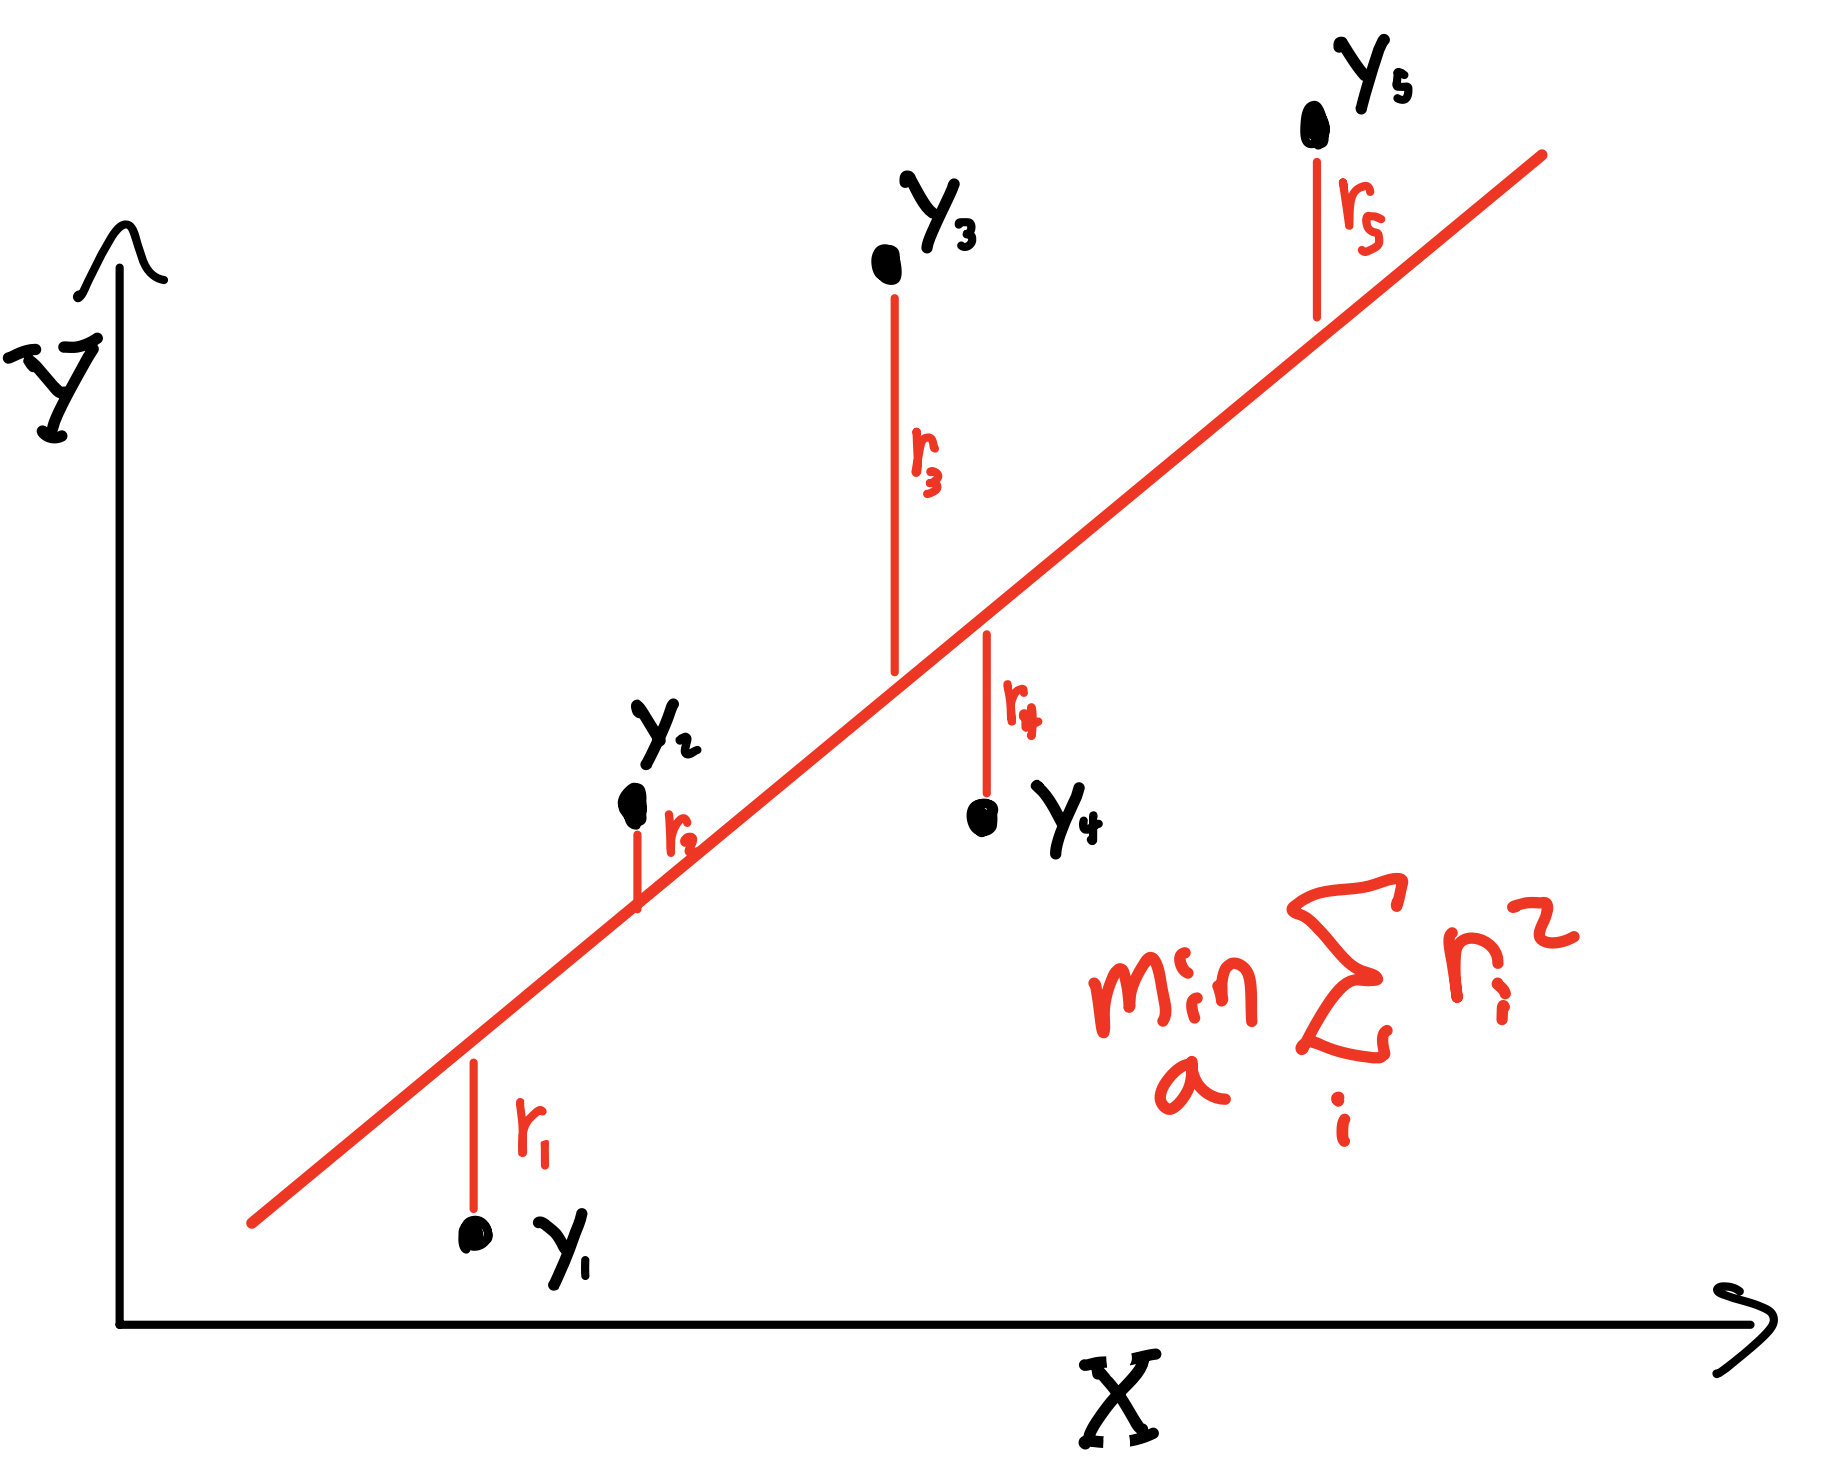
\includegraphics[width=0.4\textwidth]{./../figures/rss}
\caption{ }\label{rss}
\end{figure}


There are many other ways we could draw a line through a set of $(x,y)$ points. This particular way of estimating the slope -- by minimizing RSS -- happen to make sense under the assumption that  the data is sampled from a Linear regression model (Equation \ref{eq:linreg}). 



 % ------------------------------------------------------------------------------------------------------------------------------------------
\begin{example}[Marketing data]
Here we consider the some on advertising budgets and sales for a company. We will explore whether the budget for TV advertisements is associated with higher sales. \\

 \noindent
\underline{Questions:} Fit the data to a linear regression model with the TV budget at the  predictor and sales as the response variable. 
\begin{enumerate}[label=(\alph*)]
\item {\bf Fit linear regression model:} What are the estimates of $\beta_1$ and $\beta_0$? 
\item {\bf Visualize the data:} Plot the regression long along with a scatter plot of the data. 
%\item {\bf A rudimentary hypothesis test:}  Suppose that in reality, $\beta_1=0$. This means $\beta_0 = \mu_y$ since 
%\begin{equation*}
%\mu_y = E[Y] = \beta_1 \mu_x + \beta_0 = \beta_0.
%\end{equation*}
%Estimate $\mu_y$ and simulate $10000$ ``fake'' data sets under the assumption that $\beta_0$. For each one, estimate the slope and save it in an array. Based on these estimates, what is the chance that we obtain a value of $\beta_1$ which is at least at large as the one we obtained from the real data? This will tell us if it is possible our estimated $\hat{\beta_1}$ is positive only by accident. 
\item {\bf Accessing model assumptions:} Using the fitted values of $\beta_1$ and $\beta_0$, simulate $10$ ``fake'' data sets which have the same number of points as the real data set and the same $x$ values.  Make plots of these and compare to the real data.  \\
\end{enumerate}

 \noindent
\underline{Solution:} see \href{https://colab.research.google.com/drive/1_4zOruAWfJ3HQoIf9sjefk3z0APko94-?usp=sharing}{colab} notebook. 
\end{example}








%
%
%%------------------------------------------------------------------------------------------------------------------------------------------------------
%\section{Statistical inference for regression model using python}
%
%% NOTE: Maybe move earlier problem about ballpark estimate in test score model here
%\begin{itemize}
%\item Having introduced the concepts and terminology of statistical inference, we return to the linear regression model with a single predictor:
%\begin{align*}
%Y|X \sim {\rm Normal}(\beta_0 + \beta_1X,\sigma^2).
%\end{align*}
%We will sometimes write such a model as
%\begin{equation*}
%Y = \beta_0 + \beta_1X + \varepsilon
%\end{equation*}
%where it is assumed that 
%\begin{equation*}
%\varepsilon \sim {\rm Normal}(0,\sigma^2)
%\end{equation*}
%Note that this model does not describe the distribution of $Y$, rather it describes the distribution of $Y$ given $X$. What we are really saying is that once we are given a value of $X$, the variation in $Y$ is approximately normal with an $X$ independent variance. The formulas for estimators of $\beta_0$ and $\beta_1$ have already been given. You can look up formulas for the standard errors in the textbook, we will just have Python give us these. 
%Note that the sample distributions of $\hat{\beta}_0$ and $\hat{\beta}_1$ are NOT normal, but we will not worry about trying to compute them in this class (at least for now). 
%\item In addition, we want to estimate $\sigma^2$. To do so, we can note that 
%\begin{equation*}
%Y - (\beta_0 +\beta_1X) \sim {\rm Normal}(0,\sigma^2).
%\end{equation*}
%Therefore, with our estimates  $\hat{\beta}_0$ and $\hat{\beta}_1$, we can compute the residuals of each data point
%\begin{equation*}
%r_i = Y_i  -  (\hat{\beta}_0 +\hat{\beta}_1X_i).
%\end{equation*}
%An estimate of $\sigma^2$ is approximately the sample variance of $r_i$. We need to account for the fact that we don't know $\beta_0$ and $\beta_1$ exactly though (just like with Bessels correction), and therefore the unbiased estimator is
%\begin{equation*}
%\hat{\sigma}^2= \frac{1}{n-2} \sum_{i=1}^nr_i^2. 
%\end{equation*}
%We will refer to the process of computing the coefficient estimates and standard errors as \dfn{fitting} the model. 
%
%
%\item   In order to perform statistical inference for a linear regression model in Python, we use the \verb!statsmodels! package. \verb!statsmodels! has a function \verb!OLS! which can take two arguments
%\begin{itemize}
%\item An array \verb!y! -- the response variables
%\item and a matrix \verb!X! -- which contains the predictors. 
%\end{itemize}
%Technically,  \verb!OLS! will create a regression model of the form 
%\begin{equation*}
%Y = \beta_0 X_0 + \beta_1 X_1 + \beta_2 X_2 +\cdots + Z
%\end{equation*}
%where $Z$ is mean zero normal. Notice there is not intercept, instead we have a term $\beta_0 X_0$. We need to trick  \verb!OLS!
%into creating a model with a single predictors AND an intercept by creating a new predictor $X_0$ which is always one. This is achieved with the line of code
%\begin{Verbatim}
%X = sm.add_constant(x)
%\end{Verbatim}
%where $x$ is jus the array of our $X$ values (playing the role of $X_1$ in the equation above). 
%Then 
%\begin{Verbatim}
%model = sm.OLS(y,X)
%\end{Verbatim}
%create a model ``object''. At this point we haven't actually performed any inference, rather we have created an data structure, called an object, which has all the information about our model and data. The next step is to tell python to fit this model -- that is, to infer the parameter values -- and store the results. This is done via
%\begin{Verbatim}
%results = model.fit(). 
%\end{Verbatim}
%Results contains all the information about the fitted model, including the inferred, or fitted, coefficients, standard errors, as well as many things I will soon discuss. We can print all this out with the line of code 
%\begin{Verbatim}
%print(results.summary())
%\end{Verbatim}
%This will produce something like
%\begin{Verbatim}
%                            OLS Regression Results                            
%==============================================================================
%Dep. Variable:                      y   R-squared:                       0.612
%Model:                            OLS   Adj. R-squared:                  0.610
%Method:                 Least Squares   F-statistic:                     312.1
%Date:                Thu, 05 Oct 2023   Prob (F-statistic):           1.47e-42
%Time:                        12:43:13   Log-Likelihood:                -519.05
%No. Observations:                 200   AIC:                             1042.
%Df Residuals:                     198   BIC:                             1049.
%Df Model:                           1                                         
%Covariance Type:            nonrobust                                         
%==============================================================================
%                 coef    std err          t      P>|t|      [0.025      0.975]
%------------------------------------------------------------------------------
%const          7.0326      0.458     15.360      0.000       6.130       7.935
%x1             0.0475      0.003     17.668      0.000       0.042       0.053
%==============================================================================
%Omnibus:                        0.531   Durbin-Watson:                   1.935
%Prob(Omnibus):                  0.767   Jarque-Bera (JB):                0.669
%Skew:                          -0.089   Prob(JB):                        0.716
%Kurtosis:                       2.779   Cond. No.                         338.
%==============================================================================
%\end{Verbatim}
%The value of \verb!const! is the intercept $\beta_0$ and \verb!x1! is the coefficient of $X$ in our regression model -- that is, the slope $\beta_1$. You can access the various quantities directly from the results object via the commands in Table \ref{tab:sm}.
%
%\begin{table}[h]
%\centering
%\begin{tabular}{lr}
%\textbf{quantity} & \textbf{Command}  \\
%\hline
%\hline
%$\beta_i$ &  \verb!results.params! \\
%$\hat{\sigma}^2$ &  \verb!results.scale! \\
%${\rm se}(\hat{\beta}_i)$  & \verb!results.bse! \\
%\end{tabular}
%\caption{}
%\label{tab:sm}
%\end{table}
%
%
%
%\begin{example}[Performing linear regression in statsmodels]
%
%Here we once again consider the some on advertising budgets and sales for a company.\\
%
%
%
%\noindent
%\underline{Question:} Fit the data to a linear regression model using \verb!statsmodels! and compare to the results we got before. \\ 
%
%
%\end{example}
%\end{itemize}
%
%\subsection{Assessing explanatory power with $R^2$}
%\begin{itemize}
%\item We have so far seen how to estimate and interpret the parameters in the regression model with one predictor). So far, most of the quantities we compute depend heavily on the intrinsic scales of the data. For example, if we are working with height data as our predictor and use units of inches, we will get very different values of $\hat{\beta}_1$ than if we had used feet. The same is true for the other parameters. It is therefore useful to have a summary of the descriptive power of our model in terms of a quantity that does not depend on these scales. %Recall that the covariance is one way to measure. 
%\item To find an appropriate metric for accessing the descriptive power of our model, the idea is to compare the variation in $Y$ over all (that is, the marginal variance), to the variation conditioned on $X$. To this end, we define the \dfn{correlation coefficient} by 
%\begin{equation}
%\rho^2 = 1 - \frac{{\rm var}(Y|X)}{{\rm var}(Y)} = 1 - \frac{\sigma^2}{\beta_1^2\sigma^2 +\sigma_x^2} \approx R^2
%\end{equation}
%The quantity called $R^2$ is simply the estimator of this with all the quantities above replaced by their sample estimates:
%\begin{equation*}
%R^2 = 1 - \frac{\sum_{i=1}^nr_i^2}{\sum_{i=1}^n (Y_i - \overline{Y})^2}
%\end{equation*}
%\item There is a relationship between $\rho$ and the covariance 
%\begin{equation*}
%\rho = \frac{{\rm cov}(X,Y)}{\sigma_x\sigma_y}. 
%\end{equation*}
%I'll leave it as an exercise to show this. This provides provides another interpretation of $\rho$ (and hence $R^2$) which comes from one of the earlier exercises. In particular, if $\beta_1$ and $\beta_1'$ are respectively the regression slopes of $Y$ vs. $X$ and $X$ vs. $Y$, we can then write $\rho$ as 
%\begin{equation*}
%\rho  =  \frac{{\rm cov}(X,Y)}{\sigma_x\sigma_y} =  \frac{{\rm sign}(\beta_1)\sqrt{\beta_1'\beta_1}\sigma_x\sigma_y}{\sigma_x\sigma_y} = {\rm sign}(\beta_1)\sqrt{\beta_1'\beta_1}. 
%\end{equation*}
%
%
%\begin{example}[Performing linear regression in statsmodels]
%
%
%\noindent
%\underline{Question:} Generate simulated data with different values of $R^2$ \\ 
%
%\noindent
%\underline{Solution:} See python notebook. \\ 
%\end{example}
%
%\end{itemize}
%



%------------------------------------------------------------------------------------------------------------------------------------------------------
\section{Hypothesis testing}
In statistics, we might infer parameters not because we are interested in specific values, but rather because we would like to use them to make a decision. For example, in a clinical trial, we might be interested in deciding whether a candidate drug is worth moving forward with. This problem is often framed in terms of \dfn{hypothesis testing}, in which we assign a probability to a particular hypothesis or its converse. 
In rather abstract terms, the basic procedure of hypothesis testing is as follows:
\begin{enumerate}
\item Come up with a \dfn{null hypothesis}. For example, this might be that the mean of some variable is zero. We are interested in determining whether we can rule this hypothesis out. 
\item Compute something called a \dfn{test statistic}, denoted $\hat{T}$, which like any estimator is simply some quantity we compute from our data. 
\item Next, we do a sort of probabilistic thought experiment and ask: What is the chance that we would observe a value of $\hat{T}$ at least as large as the value we measured  IF our hypothesis was in-fact true.  The result is the \dfn{$p$-value}. 
\end{enumerate}

\begin{example}[hypothesis testing for a clinical trial]
Consider the example of a clinical trial. The effect of a drug, denoted $Y$ (e.g. blood pressure is measured in two groups) is measured in two groups.  One group is given a placebo, the other (the treatment group) is given a drug. Let $X=0$ for people in the control group and $X=2$ for those in the treatment group.   For simplicity we will assume that there are $N/2$ people in each group. We can model $Y$ with a regression model 
\begin{equation*}
Y|X \sim{\rm Normal}(\mu_C (1-X) + \mu_T X,\sigma^2)
\end{equation*}
{\bf We will assume $\sigma^2$ is know! This greatly simplifies the calculations!}
This is just a linear regression model since we could write
\begin{equation*}
\mu_C (1-X) + \mu_T X = \mu_C + (\mu_T-\mu_C)X = \beta_0 + \beta_1 X
\end{equation*}
where
\begin{align*}
\beta_0 &= \mu_C\\
\beta_1 &= \mu_T - \mu_C.
\end{align*}
We could estimate $\beta_0$ and $\beta_1$ as we always do in a linear regression model. We could also simply perform inference on the mean and of a Normal distribution within each group to obtain estimators of $\mu_C$ and $\mu_T$. For simplicity, let's pretend $\sigma$ is known for simplicity. This makes things simple, because then the sample distributions are 
 \begin{align*}
 \hat{\mu}_C &\sim {\rm Normal}\left(\hat{\mu}_C,\frac{\sigma^2}{N/2}\right)\\
  \hat{\mu}_T &\sim {\rm Normal}\left(\hat{\mu}_T,\frac{\sigma^2}{N/2}\right). 
 \end{align*}
 
Thus the (estimated) sample distribution of $\beta_1$ is 
\begin{equation*}
\hat{\beta}_1 \sim {\rm Normal}\left(\hat{\beta},\frac{4\sigma^2}{N}\right). 
\end{equation*}
In this case, our null hypothesis will be that $\beta_1  = 0$; that is, there is no effect of the drug. As our test statistic, we measure how far $\beta_1$ is from zero in standard deviations: 
\begin{equation*}
\hat{T} = \frac{\hat{\beta}_1}{{\rm se}(\hat{\beta}_1 )}
\end{equation*}
Remember that since we know $\sigma$,  ${\rm se}(\hat{\beta})$ is known and therefore, from the perspective of the sample distribution, this is just dividing by a constant. 
%Statistical significance can be understood in the language of $p$-values and hypothesis testing. The idea is that instead of looking directly at the sample distribution, we ask: How likely is it that we obtain a result at least as large as what we obtained if the null hypothesis were false. To this end, we consider the sample distribution conditioned on the null hypothesis being false:
Now, let $\hat{\beta}_1^*$ be the random variable representing the measured effect under the null hypothesis. Another way to say this is that $\hat{\beta}_1^*$ represents a measurement of $\beta_1$ from a replica generated under the assumption that $\beta_1=0$. Therefore, $\hat{\beta}_1^*$ will have a distribution centered at zero and with a standard deviation ${\rm se}(\hat{\beta}_1)$. This means the distribution of $\hat{\beta}_1^*$ is nothing but the sample distribution shifted to zero, or 
\begin{equation*}
\hat{\beta}_1^* \sim {\rm Normal}\left(0,\frac{4\sigma^2}{N}\right)
\end{equation*}
%This is a slightly different use of condition, since we are conditioning on a hypothesis, not an event in our sample. Think of it this way: the null hypothesis can itself be treated as a random variable which we are modeling 
 At this point we can answer the question posed in step 3: {\bf If the null hypothesis was true, how likely would we be to observe a value of $\hat{T}$ larger than the one we did?} This is determined by the $p$-value:
\begin{equation}\label{eq:pval}
p_v = P(|\hat{T}^*|>|\hat{T}||\hat{T})
\end{equation}
where $\hat{T}^*$ is the test statistic computed from $\hat{\beta}_1^*$ and the probability is taken over all the distribution of $\hat{T}^*$, while $\hat{T}$ is given by our data (hence why I use the conditioning notation). $p_v$, like $\hat{T}$, is a function of the data. See the python notebook were we compute $p_v$ with simulations. 

\end{example}

 The above example is very simple because we assume that $\sigma$ is known and we have only a binary predictor. In reality, the computation of $p$-values is much more complex, however the principle and interpretation is the same!
 {\bf Interpreting the $p$-value} If the $p$-value is very small, then it is highly unlikely we would have observed what we did when the null hypothesis was true. In this case, we can REJECT the null hypothesis as false. Usually some threshold is set for this, and if the $p_v$ is below that threshold we say our result in statistically significant. On the other hand, {\bf if $p_v$ is not small, it does not necessarily mean the null hypothesis is true.} A result is said to be statistically significant if $p_v<0.05$. Visually, we can see that $\beta_1$ is statistically significant exactly if $0$ is not contained in the confidence interval! 
{\bf Relationship between $p$-values and confidence intervals}.  The $p$-value is all about the ``tail'' of the sample distribution -- ``tail'' usually just means the ends of the distribution. Naturally there is connection between between $p$-values and confidence intervals, which also measure the width of the sample distribution. To illustrate the connection, we will again assume {\bf $\sigma$ is known}.  Since the  the sample distribution can be obtained by shifting the distribution of $\hat{\beta}_1^*$ to $\hat{\beta}_1$, the $p$-value, $p_v$, is exactly the chance of being outside the interval $[\hat{\beta}_1 - |\hat{\beta}_1|,\hat{\beta}_1 + |\hat{\beta}_1|]$. Therefore,  recalling the interpretation of confidence intervals, $\hat{\beta}_1$ will fall in the confidence interval with probability $p_v$ when the null hypothesis is true.  If $\sigma$ isn't known all this is only approximately true, but intuition is still. 



\begin{figure}[h]
\centering
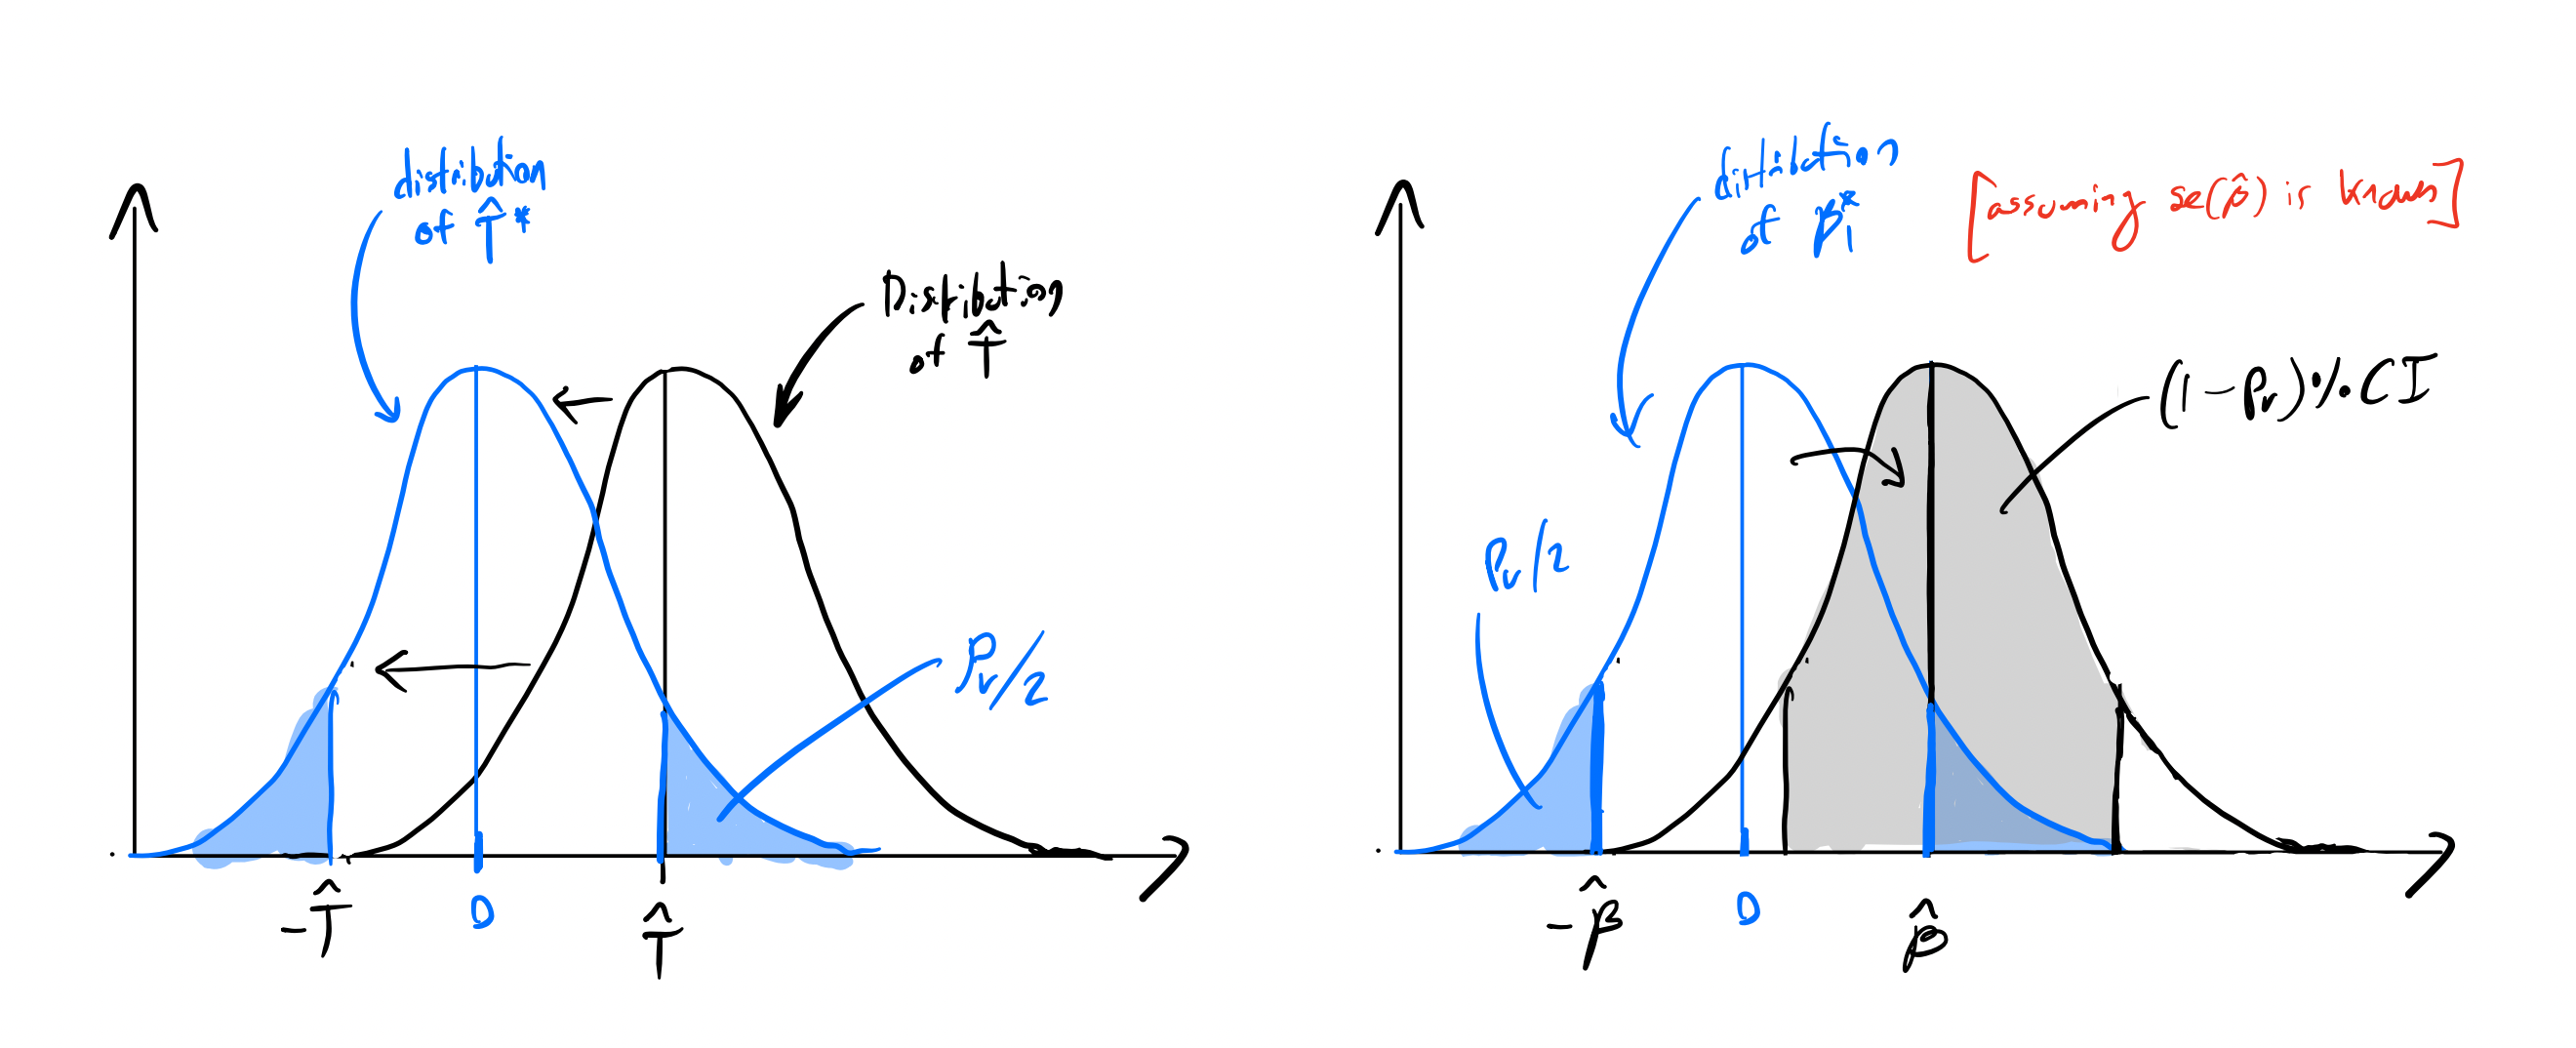
\includegraphics[width=0.8\textwidth]{./../figures/pvalueCI}
\caption{(left) The (two-sided) $p$-value and (right) the relationship between $p_v$ and the confidence interval. }\label{fig:pvalue}
\end{figure}




\newpage

\section*{Exercises}
 % ------------------------------------------------------------------------------------------------------------------------------------------
\begin{exercise}[Bias and consistency]\label{ex:1}
Let
\begin{equation*}
X \sim {\rm Bernoulli}(q)
\end{equation*}
and $X_1,\dots,X_N$ denote $N$ samples of $X$. 
For each of the following estimators of $q$, (i) write down the standard error and (ii) state whether they are un-biased and/or consistent. (In each case, you can write down an exact formula for the standard error, so you do NOT need to use the CLT.)
\begin{enumerate}[label=(\alph*)]
\item 
\begin{equation*}
\hat{q}_{0} = \frac{1}{N}\sum_{i=1}^NX_i
\end{equation*}
\item 
\begin{equation*}
\hat{q}_{1} = \frac{Y}{N} + \frac{1}{\sqrt{N}},\quad Y = \sum_{i=1}^NX_i
\end{equation*}
\item 
\begin{equation*}
\hat{q}_{2} = \frac{1}{\lfloor N/2 \rfloor}\sum_{i=1}^{\lfloor N/2 \rfloor}X_i
\end{equation*}
The notation $\lfloor  n \rfloor$ means the floor; that is, the largest integer less than $n$. For example, $\lfloor 101/2 \rfloor = \lfloor 50.5 \rfloor = 50$. 
\end{enumerate}

\end{exercise}




 % ------------------------------------------------------------------------------------------------------------------------------------------

 % ------------------------------------------------------------------------------------------------------------------------------------------
%\begin{exercise}{\bf bias}
%Let $q$ be the parameter of a Bernoulli random variable. Let $\hat{q}$, $\hat{q}_1$ and $\hat{q}_2$ be two other estimators of $q$ defined by \begin{align}
%\hat{q} &= \frac{Y}{N}\\
%\hat{q}_{1} &= \frac{Y}{N} + \frac{1}{N}\\
%\hat{q}_{2} &= \frac{y_1 + y_2}{2}
%\end{align}
%\begin{enumerate}
%\item What are the sample distributions of these? 
%\item Are they consistent?
%\item Are they biased?
%\item Confirm your answers with simulations. 
%\end{enumerate}
%%Are $\hat{q}_1$ and $\hat{q}_2$ biased or not? Try to answer the question based solely on the definitions and generate simulations and make a plot (or multiple plots) to support your result. {\emph Hint:} Think about what the sample distribution of these estimators are.
%\end{exercise}


 % ------------------------------------------------------------------------------------------------------------------------------------------
\begin{exercise}[Estimator of mean in exponential model]
Let
\begin{equation*}
T \sim {\rm Exponential}(\lambda). 
\end{equation*}
Recall that $E[T] = 1/\lambda$. We can estimate $E[T]$ via the sample average of measurements $T_1,\dots,T_n$, 
\begin{equation*}
E[T] \approx \overline{T} = \frac{1}{n}\sum_{i=1}^nT_i.
\end{equation*}
This suggests that a natural way to estimate $\lambda$ is by 
\begin{equation*}
\hat{\lambda} = \frac{1}{\overline{T}} = \frac{1}{ \frac{1}{n}\sum_{i=1}^nT_i}. 
\end{equation*}
\begin{enumerate}[label=(\alph*)]
\item  The goal of the first part of this problem is to show, using simulations, that this is in-fact a biased estimator of $\lambda$, although the bias decreases with $n$. 
To achieve this, you should do the following: 
\begin{itemize}
\item Make a list of 100 values of $\lambda$. You could use any range, but I picked between $0.2$ and $2$. 
\item For each value of $\lambda$, 
\begin{itemize}
\item simulate $10000$ replicates of an experiment, where each replicate includes $n=5$ values of $T$. 
\item For each of these replicates, compute $\hat{\lambda}$ as defined above. 
\item Then estimate the average $E[\hat{\lambda}]$ and save this value in a list. 
\end{itemize}
\item Make a plot of $\lambda$ vs. $\left|E[\hat{\lambda}]-\lambda\right|$. 
\end{itemize}
\item ({\bf optional -- ungraded}) Consider the case $n=2$. Prove that 
\begin{equation*}
E[\hat{\lambda}] = E\left[\frac{1}{\overline{T}}\right]  \ge \lambda 
\end{equation*}
This is a special case of Jenson's inequality. 
\end{enumerate}


%Consider the non-linear model
%\begin{align}
%Y &= X^2 + \epsilon \\
%X &\sim {\rm Normal}(0,1)\\
%\epsilon &\sim {\rm Normal}(0,\sigma_{\epsilon})
%\end{align}
%\begin{enumerate}
%\item Is the distribution of $Y$ Normal? You do not need to determine what the distribution is to answer this. 
%\item What about the distribution of $Y|(X=x)$? 
%\item What about the covariance?
%\end{enumerate}
\end{exercise}





 % ------------------------------------------------------------------------------------------------------------------------------------------
\begin{exercise}[Earnings data] Consider the earnings data. This can be loaded with 
\begin{Verbatim}
df = pd.read_csv("https://raw.githubusercontent.com/avehtari
/ROS-Examples/master/Earnings/data/earnings.csv")
\end{Verbatim}
In this exercises, you will study the association between earnings and gender. In particular, you will explore how this depends on height. Later we will see there is a better way to answer this question by performing a regression with multiple predictors, but taking this more elementary approach will elucidate some key aspects of regression analysis. 
\begin{enumerate}[label=(\alph*)]
\item What do you expect the association between gender and earnings to be? Where do you expectations come from (news, intuition, other courses you've taken)? 
\item Using stats models, perform a linear regression on with gender (the column ``male'') as the predictor and earnings as the response variable. You can either use ``earnk'' or ``earn'', just keep track of the units.  Then answer the questions 
\begin{itemize}
\item Is there a statistically significant effect? 
\item Is the direction and size of the effect what you expected? 
\end{itemize}
\item  Using stats models, perform a linear regression with height as the predictor and earnings as the response variable. Answer the same questions which are posed in part (a). 
\item You should have found there is an association between both gender and earnings, as well as height and earnings. 
 A natural question is whether the association between height and earnings is simply a byproduct of the fact that men are taller on average.  To answer this question, separate the data into males and females, then fit the linear regression model with height as a predictor separately for each group. 
 \item Based on the results from the previous problem, what do you conclude? Is the association between height and earnings solely due to the association between gender and heights? Do you think it is partially due to the height? 
\end{enumerate}
\end{exercise}

 % ------------------------------------------------------------------------------------------------------------------------------------------
\begin{exercise}[Quiz practice]
Answer the questions on the practice quiz. You are welcome to provide some feedback on the quiz regarding difficultly level, clarity of problems, relevance to course material etc. 
\end{exercise}



 % ------------------------------------------------------------------------------------------------------------------------------------------
\begin{exercise}[Statistical significance -- {\bf optional challenge}]
Show (using math OR simulations) that it is possible to conduct two experiments (let's use clinical trials as an example) so that $\Delta \hat{\mu}$ (using the same notation as my notes) is statistically significant for one experiment and not the other, yet the difference between $\Delta \hat{\mu}$ between the two experiments is not statistically significant.  Here, by statistically significant I mean the $p$-value is $<0.05$. 
\end{exercise}





 \bibliographystyle{unsrt}
\bibliography{./../refs.bib}

\end{document}


% WHAT IS THIS? 
\subsection{A simple example}
\begin{itemize}
\item Now let's consider the general regression model
\begin{equation}
Y = aX + b + \epsilon 
\end{equation}
where $X$ may be a continuous variable. 
{\bf How would we estimate $a$? }
\item Let's look at a simple example: 
Consider the example of a clinical trial conducted as follows. Suppose $N$ people participate in the trial, and are randomly assigned to the the control group (C) and treatment group (T) with probability $1/2$. People in T are given a drug whose effects is measure by a percent.  
\item We can model the distribution of blood pressure before and after treatment as 
\begin{equation}
Y_C \sim {\rm Normal}(\mu_C,\sigma)
\end{equation}
and 
\begin{equation}
Y_T \sim {\rm Normal}(\mu_T,\sigma).
\end{equation}
\item Our model for an individuals response can be framed as a regression model 
\begin{equation}\label{eq:clinical}
Y  = (\mu_T-\mu_C)X + \mu_C + \epsilon
\end{equation}
where $X=1$ if someone is in the treatment group and 
\begin{equation}
\epsilon \sim {\rm Normal}(0,\sigma_{\epsilon}). 
\end{equation}
\item How would we estimate $\mu_T$, $\mu_C$ and $\sigma$ from a sample? Assuming we know the group each patient has been assigned to, we observe that 
\begin{equation}
\E[Y|X=1] = \mu_T,\quad  \sqrt{{\rm var}(Y|X=1)} = \sigma_{\epsilon}. 
\end{equation}
This means we can estimate these from sample averages of $Y$ and $X$ (and similar for $X=0$).
%\begin{boxA}{$\sigma_{\epsilon}$ vs. $\sigma$}
% You might be tempted to say that the variance of $Y$ is also $\sigma_{\epsilon}$ -- but this is false! Why? (think back to the previous note when we looked at the marginal distribution of $Y$)
\item The sample distribution of the mean of the treatment group is
\begin{equation*}
\hat{\mu}_T \sim {\rm Normal}\left(\mu_T,\sigma/\sqrt{N}\right)
\end{equation*}
If  $\Delta \mu = \mu_T-\mu_C$, then as estimator $\Delta \mu$ is 
\begin{equation*}
\Delta \hat{\mu} =  \hat{\mu}_T-\hat{\mu}_C
\end{equation*}
which is really the slope of the regression line. 
The sample distribution of $\Delta \hat{\mu}$ is also Normal:
\begin{equation*}
\Delta \hat{\mu} \sim {\rm Normal}\left(\Delta \mu, \sqrt{2}\sigma/\sqrt{N}\right)
\end{equation*}





%\end{boxA}
\end{itemize}







 \bibliographystyle{unsrt}
\bibliography{./../refs.bib}


\end{document}